\documentclass[border=0pt,10pt]{standalone}
\usepackage[T1]{fontenc}
\usepackage{lmodern}
\usepackage{pgfplots}
\pgfplotsset{compat=1.17}
\usepgfplotslibrary{groupplots}
\usepackage{xcolor}
\definecolor{oi-blue}{HTML}{0072B2}
\definecolor{oi-vermillion}{HTML}{D55E00}
\definecolor{oi-green}{HTML}{009E73}
\definecolor{oi-purple}{HTML}{CC79A7}
\definecolor{oi-black}{HTML}{000000}
% semantic_sha256: bd2a953e6fdeba82f892112e77e569b479863bd0d1672a21f119ca1f80c333bc
\begin{document}
\begin{minipage}{181.86mm}
\centering
{\bfseries\fontsize{10}{12}\selectfont PP-U-ARPLS | D3 | final\_refit}\\[2mm]
{\fontsize{8}{10}\selectfont planned=42, monitored=42, missing-history=0, status=complete\_history\_coverage}\\[3mm]
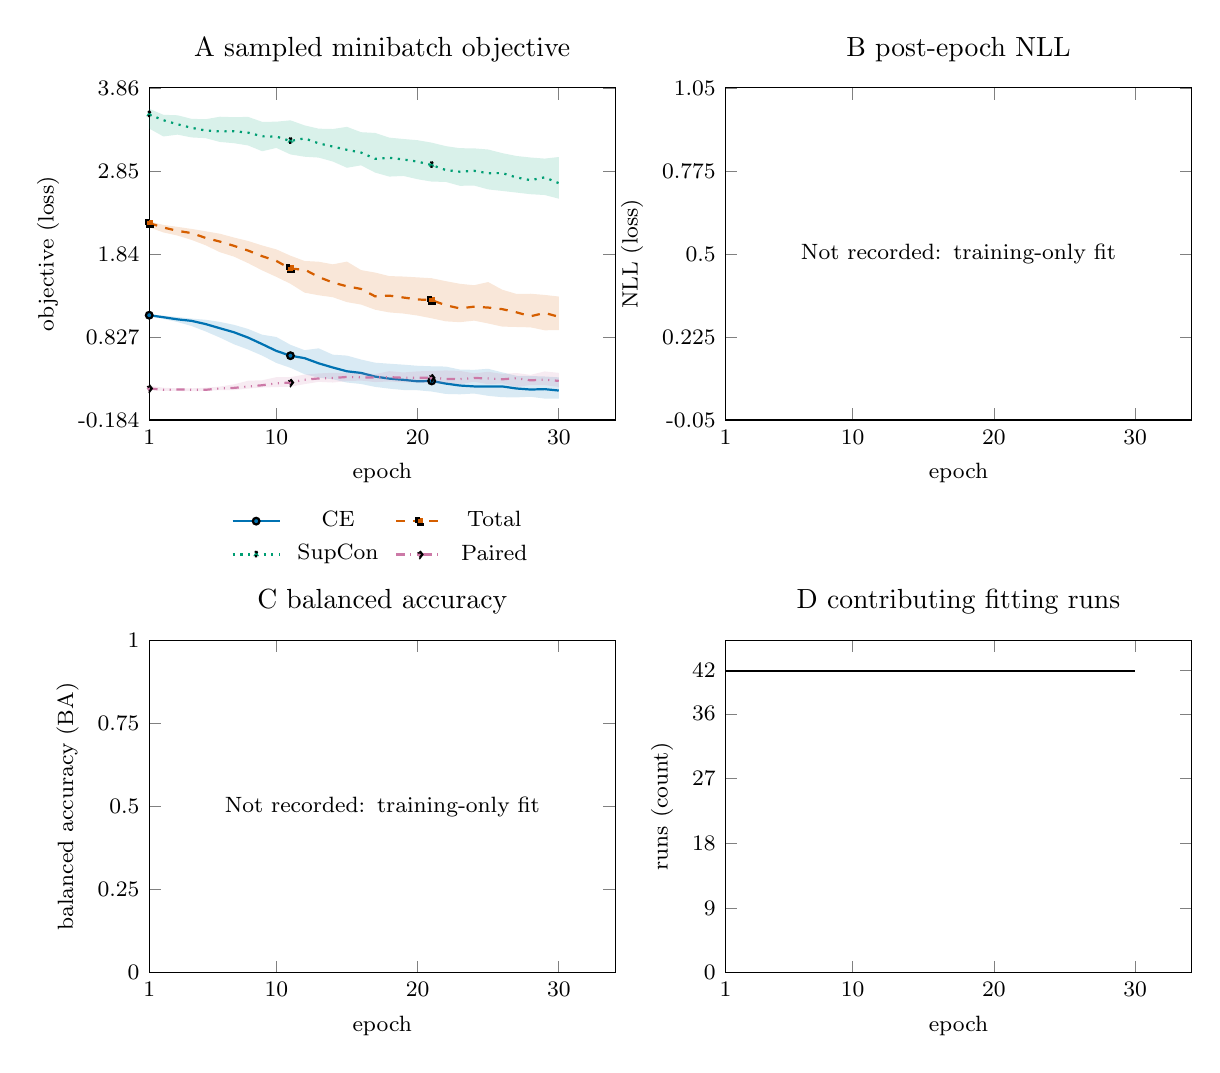
\begin{tikzpicture}
\begin{groupplot}[group style={group size=2 by 2, horizontal sep=14mm, vertical sep=28mm}]
\nextgroupplot[width=75mm, height=58mm, title={A sampled minibatch objective}, xlabel={epoch}, ylabel={objective (loss)}, xmin=1, xmax=34, xtick={1,10,20,30}, ymin=-0.18368585109710694, ymax=3.8574028730392458, ytick={-0.18368585109710694,0.82658632993698133,1.8368585109710696,2.8471306920051576,3.8574028730392458}, yticklabels={-0.184,0.827,1.84,2.85,3.86}, tick label style={font=\fontsize{8}{9}\selectfont, text=black}, label style={font=\fontsize{8}{9}\selectfont, text=black}, title style={font=\fontsize{10}{11}\selectfont, text=black}, legend style={at={(0.5,-0.24)},anchor=north,draw=none,fill=none,font=\fontsize{8}{9}\selectfont,row sep=1pt,column sep=4pt,legend columns=2}]
\addplot[fill=oi-blue,opacity=0.15,draw=none,forget plot] coordinates {(1,1.0817828625440598) (2,1.0464966624975205) (3,1.0090737611055374) (4,0.95978249758481982) (5,0.89367171376943588) (6,0.81961800307035448) (7,0.73804353922605515) (8,0.67400917708873753) (9,0.59992869943380356) (10,0.5109543614089489) (11,0.45122150182723997) (12,0.37354467660188678) (13,0.33155569434165955) (14,0.31222746446728705) (15,0.27263176366686825) (16,0.2549035385251045) (17,0.21946738064289092) (18,0.19818866606801749) (19,0.18174436036497357) (20,0.17890978455543519) (21,0.16305664833635092) (22,0.13374160900712015) (23,0.12944261673837901) (24,0.13895774316042661) (25,0.11058042095974088) (26,0.094117483310401442) (27,0.091799075156450277) (28,0.099442513659596443) (29,0.077277597691863778) (30,0.075722471624612805) (30,0.33572065308690069) (29,0.34617187678813932) (28,0.35164986774325369) (27,0.3552918307483196) (26,0.39588829427957534) (25,0.43989923372864725) (24,0.42703734785318376) (23,0.4305606678128242) (22,0.46693948954343789) (21,0.47027522101998331) (20,0.47624349668622018) (19,0.49006286486983297) (18,0.50170455351471899) (17,0.51385380625724797) (16,0.55242974162101743) (15,0.6001700080931186) (14,0.61153604984283449) (13,0.68868202865123751) (12,0.66651907861232762) (11,0.73161900788545609) (10,0.82694084048271177) (9,0.85419576615095139) (8,0.92457027882337572) (7,0.97471421957015991) (6,1.0102470681071281) (5,1.0360709726810455) (4,1.0501629024744035) (3,1.0688730716705321) (2,1.086257165670395) (1,1.1005660086870193)};
\addplot[color=oi-blue, mark=*, mark options={draw=black}, mark repeat=10, mark size=1.2pt, solid, line width=0.8pt] coordinates {(1,1.091413676738739) (2,1.0672686398029327) (3,1.0412436872720718) (4,1.0227195620536804) (5,0.98348798602819443) (6,0.9333319216966629) (7,0.88420608639717102) (8,0.81926935911178589) (9,0.73969060182571411) (10,0.65733495354652405) (11,0.59902713447809219) (12,0.56921668350696564) (13,0.50611833110451698) (14,0.45540169253945351) (15,0.40934653952717781) (16,0.38934847339987755) (17,0.34476825222373009) (18,0.32005379535257816) (19,0.30539547838270664) (20,0.28734606690704823) (21,0.29179906286299229) (22,0.2599467933177948) (23,0.23599395900964737) (24,0.22557591460645199) (25,0.22434837650507689) (26,0.22498888801783323) (27,0.20017399825155735) (28,0.18738135509192944) (29,0.19236608408391476) (30,0.17491963692009449)};
\addlegendentry{CE}
\addplot[fill=oi-vermillion,opacity=0.15,draw=none,forget plot] coordinates {(1,2.1607217729091643) (2,2.0988848149776458) (3,2.0606318056583404) (4,2.007606717944145) (5,1.9418164581060409) (6,1.8583184123039245) (7,1.8044225007295609) (8,1.7249707311391831) (9,1.6365626484155655) (10,1.5581405371427537) (11,1.4738036096096039) (12,1.3659681379795074) (13,1.3341780185699463) (14,1.3104421913623809) (15,1.2507096707820893) (16,1.221166443824768) (17,1.1580787599086761) (18,1.1255800545215606) (19,1.1117728322744369) (20,1.0873657256364821) (21,1.053947526216507) (22,1.0170006632804871) (23,1.0067295551300048) (24,1.0254917368292809) (25,0.99101502746343617) (26,0.95312244892120368) (27,0.94820654094219203) (28,0.94362124055624008) (29,0.90859878510236736) (30,0.90886045396327975) (30,1.3188210397958755) (29,1.3384248644113541) (28,1.3527768522500991) (27,1.3508635759353638) (26,1.4019045501947403) (25,1.4949709922075272) (24,1.4564935237169265) (23,1.4738987386226654) (22,1.506205928325653) (21,1.5414810448884964) (20,1.551934152841568) (19,1.5621121525764465) (18,1.5676849126815795) (17,1.6101915240287781) (16,1.6406942695379256) (15,1.7438435792922973) (14,1.7108056396245956) (13,1.7423799753189086) (12,1.7514544546604156) (11,1.8155580759048462) (10,1.8924946814775467) (9,1.940067532658577) (8,1.994847869873047) (7,2.0367517054080961) (6,2.0832621693611144) (5,2.1126805186271667) (4,2.1413840711116792) (3,2.1665187418460845) (2,2.1900098621845245) (1,2.2338203907012941)};
\addplot[color=oi-vermillion, mark=square*, mark options={draw=black}, mark repeat=10, mark size=1.2pt, dashed, line width=0.8pt] coordinates {(1,2.2120907604694366) (2,2.1588160395622253) (3,2.1175514459609985) (4,2.0910370051860809) (5,2.0314448922872543) (6,1.987633615732193) (7,1.9355624169111252) (8,1.8780798763036728) (9,1.8093134164810181) (10,1.752487525343895) (11,1.6565029621124268) (12,1.64725062251091) (13,1.5563221275806427) (14,1.4892467558383942) (15,1.4432392865419388) (16,1.4112794399261475) (17,1.320614218711853) (18,1.3296826332807541) (19,1.3068236410617828) (20,1.2831540554761887) (21,1.2750012427568436) (22,1.2128565162420273) (23,1.1745141297578812) (24,1.1956053823232651) (25,1.1845956966280937) (26,1.1652189940214157) (27,1.1270846053957939) (28,1.0784971863031387) (29,1.1192223280668259) (30,1.0727601200342178)};
\addlegendentry{Total}
\addplot[fill=oi-green,opacity=0.15,draw=none,forget plot] coordinates {(1,3.3625796139240265) (2,3.2662058174610138) (3,3.2883853971958161) (4,3.2544388771057129) (5,3.2455488562583925) (6,3.199534225463867) (7,3.1844032585620878) (8,3.1568756043910979) (9,3.0863949179649355) (10,3.1268550276756288) (11,3.0476952672004698) (12,3.0197882950305939) (13,3.0090945601463317) (14,2.9612725973129272) (15,2.8853907227516173) (16,2.9149415850639344) (17,2.8265126228332518) (18,2.7782192766666411) (19,2.7856921672821047) (20,2.7461593866348268) (21,2.7171744704246521) (22,2.7133588194847107) (23,2.6657697677612306) (24,2.6692823112010955) (25,2.6221551597118378) (26,2.6035159945487978) (27,2.5838352620601652) (28,2.56372931599617) (29,2.5538675844669343) (30,2.5095756292343139) (30,3.0163916289806365) (29,2.9969788432121276) (28,3.0101513385772702) (27,3.0288809657096865) (26,3.0636310696601869) (25,3.107330548763275) (24,3.1216592609882352) (23,3.1234191000461577) (22,3.1487430810928343) (21,3.1912414073944091) (20,3.2206958949565889) (19,3.2355298757553101) (18,3.2520176768302917) (17,3.3088902890682221) (16,3.3183059275150297) (15,3.3833200335502625) (14,3.3567733705043792) (13,3.3610493481159209) (12,3.401129198074341) (11,3.4627420186996458) (10,3.4457606434822083) (9,3.4441699564456938) (8,3.5044494450092314) (7,3.5008245289325712) (6,3.5063686430454255) (5,3.476014184951782) (4,3.4806012213230133) (3,3.5238126695156096) (2,3.5300836682319643) (1,3.6029891848564146)};
\addplot[color=oi-green, mark=triangle*, mark options={draw=black}, mark repeat=10, mark size=1.2pt, dotted, line width=0.8pt] coordinates {(1,3.5337666571140289) (2,3.463794618844986) (3,3.4147281646728516) (4,3.3713166415691376) (5,3.3384685814380646) (6,3.327286571264267) (7,3.3300449848175049) (8,3.312616229057312) (9,3.2678666710853577) (10,3.2650006413459778) (11,3.2107029855251312) (12,3.2433253824710846) (13,3.1822468042373657) (14,3.1431839764118195) (15,3.1036704182624817) (16,3.0706002414226532) (17,2.9945473670959473) (18,3.006966233253479) (19,2.9860678315162659) (20,2.9606809914112091) (21,2.9185642004013062) (22,2.857765257358551) (23,2.8374832570552826) (24,2.8483937978744507) (25,2.8191445171833038) (26,2.8207131922245026) (27,2.7680236101150513) (28,2.7345114052295685) (29,2.768902450799942) (30,2.6982851028442383)};
\addlegendentry{SupCon}
\addplot[fill=oi-purple,opacity=0.15,draw=none,forget plot] coordinates {(1,0.17984517179429532) (2,0.17219838537275792) (3,0.17049576267600058) (4,0.16749170683324338) (5,0.17012574709951878) (6,0.18086351044476032) (7,0.18029648549854754) (8,0.19879983887076377) (9,0.21204483658075332) (10,0.21738176383078098) (11,0.22218717411160469) (12,0.25302483029663564) (13,0.28095476813614367) (14,0.27250948064029218) (15,0.2898657165467739) (16,0.29664151333272459) (17,0.27782353572547436) (18,0.28561309389770029) (19,0.27477342970669272) (20,0.27272145375609397) (21,0.26381285041570662) (22,0.26720447167754174) (23,0.25307399034500122) (24,0.28235907629132273) (25,0.25171172805130482) (26,0.26234000585973261) (27,0.21897628866136074) (28,0.24209996350109578) (29,0.2411203619092703) (30,0.21935525201261044) (30,0.39058894179761405) (29,0.40755637884140011) (28,0.36565876677632331) (27,0.38825345486402513) (26,0.3777221992611885) (25,0.40314850583672523) (24,0.3847781181335449) (23,0.41378368251025677) (22,0.41971910074353214) (21,0.41409681215882299) (20,0.40843008905649181) (19,0.39508230388164517) (18,0.41119711175560947) (17,0.37560138329863546) (16,0.39276432618498802) (15,0.39118758961558342) (14,0.39126446321606634) (13,0.38330886140465736) (12,0.36942462734878062) (11,0.33852119855582713) (10,0.33777474202215668) (9,0.30021250434219837) (8,0.2946756441146135) (7,0.25054410472512245) (6,0.22326277978718281) (5,0.20910175591707228) (4,0.20217122696340084) (3,0.20131781920790673) (2,0.20942604579031468) (1,0.23248520605266093)};
\addplot[color=oi-purple, mark=diamond*, mark options={draw=black}, mark repeat=10, mark size=1.2pt, dash dot dot, line width=0.8pt] coordinates {(1,0.20027247071266174) (2,0.18464129231870174) (3,0.18759378790855408) (4,0.18548532202839851) (5,0.1841864250600338) (6,0.20061361230909824) (7,0.20752667263150215) (8,0.22346257045865059) (9,0.23980844765901566) (10,0.26288940198719501) (11,0.27224688231945038) (12,0.30706262961030006) (13,0.32235221564769745) (14,0.32686637155711651) (15,0.34043611586093903) (16,0.33506547659635544) (17,0.33503837697207928) (18,0.337724968791008) (19,0.33078309148550034) (20,0.33023160323500633) (21,0.33066614717245102) (22,0.31645519100129604) (23,0.31384306401014328) (24,0.32814900949597359) (25,0.32286467961966991) (26,0.31163774244487286) (27,0.32602032460272312) (28,0.29920517280697823) (29,0.30752371251583099) (30,0.29262101277709007)};
\addlegendentry{Paired}
\nextgroupplot[width=75mm, height=58mm, title={B post-epoch NLL}, xlabel={epoch}, ylabel={NLL (loss)}, xmin=1, xmax=34, xtick={1,10,20,30}, ymin=-0.050000000000000003, ymax=1.05, ytick={-0.050000000000000003,0.22500000000000003,0.5,0.77500000000000002,1.05}, yticklabels={-0.05,0.225,0.5,0.775,1.05}, tick label style={font=\fontsize{8}{9}\selectfont, text=black}, label style={font=\fontsize{8}{9}\selectfont, text=black}, title style={font=\fontsize{10}{11}\selectfont, text=black}]
\node[align=center, text width=55mm, font=\fontsize{8}{9}\selectfont] at (axis cs:17.5,0.5) {Not recorded: training-only fit};
\nextgroupplot[width=75mm, height=58mm, title={C balanced accuracy}, xlabel={epoch}, ylabel={balanced accuracy (BA)}, xmin=1, xmax=34, xtick={1,10,20,30}, ymin=0, ymax=1, ytick={0,0.25,0.5,0.75,1}, yticklabels={0,0.25,0.5,0.75,1}, tick label style={font=\fontsize{8}{9}\selectfont, text=black}, label style={font=\fontsize{8}{9}\selectfont, text=black}, title style={font=\fontsize{10}{11}\selectfont, text=black}]
\node[align=center, text width=55mm, font=\fontsize{8}{9}\selectfont] at (axis cs:17.5,0.5) {Not recorded: training-only fit};
\nextgroupplot[width=75mm, height=58mm, title={D contributing fitting runs}, xlabel={epoch}, ylabel={runs (count)}, xmin=1, xmax=34, xtick={1,10,20,30}, ymin=0, ymax=46.200000000000003, ytick={0,9,18,27,36,42}, yticklabels={0,9,18,27,36,42}, tick label style={font=\fontsize{8}{9}\selectfont, text=black}, label style={font=\fontsize{8}{9}\selectfont, text=black}, title style={font=\fontsize{10}{11}\selectfont, text=black}]
\addplot[color=oi-black, solid, line width=0.8pt] coordinates {(1,42) (2,42) (3,42) (4,42) (5,42) (6,42) (7,42) (8,42) (9,42) (10,42) (11,42) (12,42) (13,42) (14,42) (15,42) (16,42) (17,42) (18,42) (19,42) (20,42) (21,42) (22,42) (23,42) (24,42) (25,42) (26,42) (27,42) (28,42) (29,42) (30,42)};
\end{groupplot}
\end{tikzpicture}
\par\vspace{6mm}
\begin{minipage}{175mm}
{\fontsize{8}{10}\selectfont RQ-S01 / Scope E: descriptive training diagnostics. 400-1800 cm-1 inputs: SG uses impulse replacement and Savitzky-Golay smoothing; arPLS uses impulse replacement and baseline correction; both finish with [0,1] min-max scaling. CE = chemical cross-entropy; SupCon = supervised contrastive; Paired = paired consistency; NLL = negative log-likelihood; BA = balanced accuracy. Authenticated complete monitor histories aggregated across unique fitting jobs into descriptive policy/recipe/stage curves. Curves summarize per-epoch minibatch-weighted training chemical cross-entropy and the composite total optimization objective; these sampled minibatch objectives differ from post-epoch evaluation negative log-likelihood. Auxiliary supcon/paired loss components are recipe-specific and are not directly comparable to the total objective across recipes. Validation metrics are recorded for source\_fit runs only and never substitute for a held-out test set; calibration\_model\_fit and final\_refit rows carry training-only diagnostics. Source\_fit optimization uses a 30-epoch minimum stopping threshold and a 200-epoch maximum; refit stages reuse the caller-selected duration. Curves are fitting-run-weighted descriptive summaries over correlated runs (seeds/splits). Lines show medians; 10th/90th percentiles describe variation among saved fitting runs, not confidence intervals. Only runs that reached each epoch contribute; early stopping changes the composition, and stopped runs are not carried forward. Fitting jobs are not independent chemical samples: the dataset has 598 spectra from 69 physical samples and 10 instruments. Coverage is limited to saved SG/arPLS monitor histories; historical MIN losses are not pooled or invented. A missing history is not a zero loss or proof of a failed model. These curves do not support hypothesis tests, superiority claims, model selection, or new uncertainty inference. P08 learned-method performance is reported elsewhere.}
\end{minipage}
\end{minipage}
\end{document}